\documentclass[UTF8]{ctexart}
\usepackage{amsmath, amssymb, graphicx, booktabs, geometry}
\geometry{a4paper, margin=2.5cm}

\title{TLE/SGP4轨道预报误差的统计分析}
\author{}
\date{}

\begin{document}
\maketitle

\begin{abstract}
本文基于公开TLE编目数据与SGP4传播模型，研究空间目标在1天、3天和7天预报时长下的位置误差分布及其增长规律。以较早历元TLE作为预报初值，将其传播到未来目标时刻；以目标时刻附近的新TLE传播结果作为近似参考轨道，计算三维位置误差。进一步使用Percentile Bootstrap与BCa Bootstrap对误差统计量给出置信区间，并与Gaussian近似区间比较。最后，采用ANOVA与Kruskal-Wallis检验比较LEO、MEO、GEO三类轨道目标的误差差异。
\end{abstract}

\section{研究背景}

TLE是目前最广泛使用的公开空间目标轨道根数格式，配合SGP4模型可以快速预报卫星位置。然而，TLE是基于观测数据拟合得到的平均轨道根数，并非高精度动力学轨道，预报误差会随时间积累。

\section{数据来源与预处理}

数据来源包括CelesTrak当前GP/TLE数据快照与Space-Track \texttt{gp\_history}历史TLE数据。轨道类型按轨道周期与高度划分为LEO、MEO、GEO三类。

\section{误差计算方法}

对同一NORAD目标，设较早TLE为 $T_i$，其历元为 $t_i$。对预报时长 $\Delta t \in \{1,3,7\}$ 天，目标时刻为
\[
t^\* = t_i + \Delta t.
\]
将 $T_i$ 用SGP4传播到 $t^\*$，得到
\[
\mathbf r_{\mathrm{pred}}(t^\*) = \mathrm{SGP4}(T_i, t^\*).
\]
选择同一目标在 $t^\*$ 附近的新TLE $T_j$ 作为参考，并传播到同一目标时刻：
\[
\mathbf r_{\mathrm{ref}}(t^\*) = \mathrm{SGP4}(T_j, t^\*).
\]
三维位置误差定义为
\[
E(\Delta t)=\left\|\mathbf r_{\mathrm{pred}}(t^\*)-\mathbf r_{\mathrm{ref}}(t^\*)\right\|_2.
\]

\section{协方差传播}

误差向量记为
\[
\mathbf e(t)=\mathbf r_{\mathrm{pred}}(t)-\mathbf r_{\mathrm{ref}}(t).
\]
经验协方差矩阵为
\[
\hat\Sigma(\Delta t)=\operatorname{Cov}[\mathbf e(\Delta t)].
\]
理论协方差传播形式为
\[
\Sigma(\Delta t)=\Phi(\Delta t)\Sigma_0\Phi(\Delta t)^T+Q(\Delta t).
\]
在没有额外动力学线性化模型时，可采用 $\Phi=I$ 作为经验基线。

\section{误差增长律}

本文拟合线性模型
\[
E(t)=\alpha+\beta t+\varepsilon
\]
以及幂律模型
\[
E(t)=a t^b.
\]
幂律模型可转化为
\[
\log E(t)=\log a+b\log t.
\]

\section{Bootstrap置信区间}

对每个``轨道类型 $\times$ 预报时长''的误差样本，估计均值、中位数与RMSE，并比较Gaussian近似、Percentile Bootstrap与BCa Bootstrap区间。

\section{轨道类型差异检验}

对每个预报时长分别检验LEO、MEO、GEO的误差分布差异。若满足近似正态与方差齐性，可参考单因素ANOVA；考虑到误差分布可能偏态且长尾，同时采用Kruskal-Wallis非参数检验。

\section{实验结果}

此处填入 \texttt{outputs/tables/summary.csv}、\texttt{growth\_fit.csv}、\texttt{bootstrap\_ci.csv} 和 \texttt{group\_tests.csv} 的结果。

\begin{figure}[htbp]
\centering
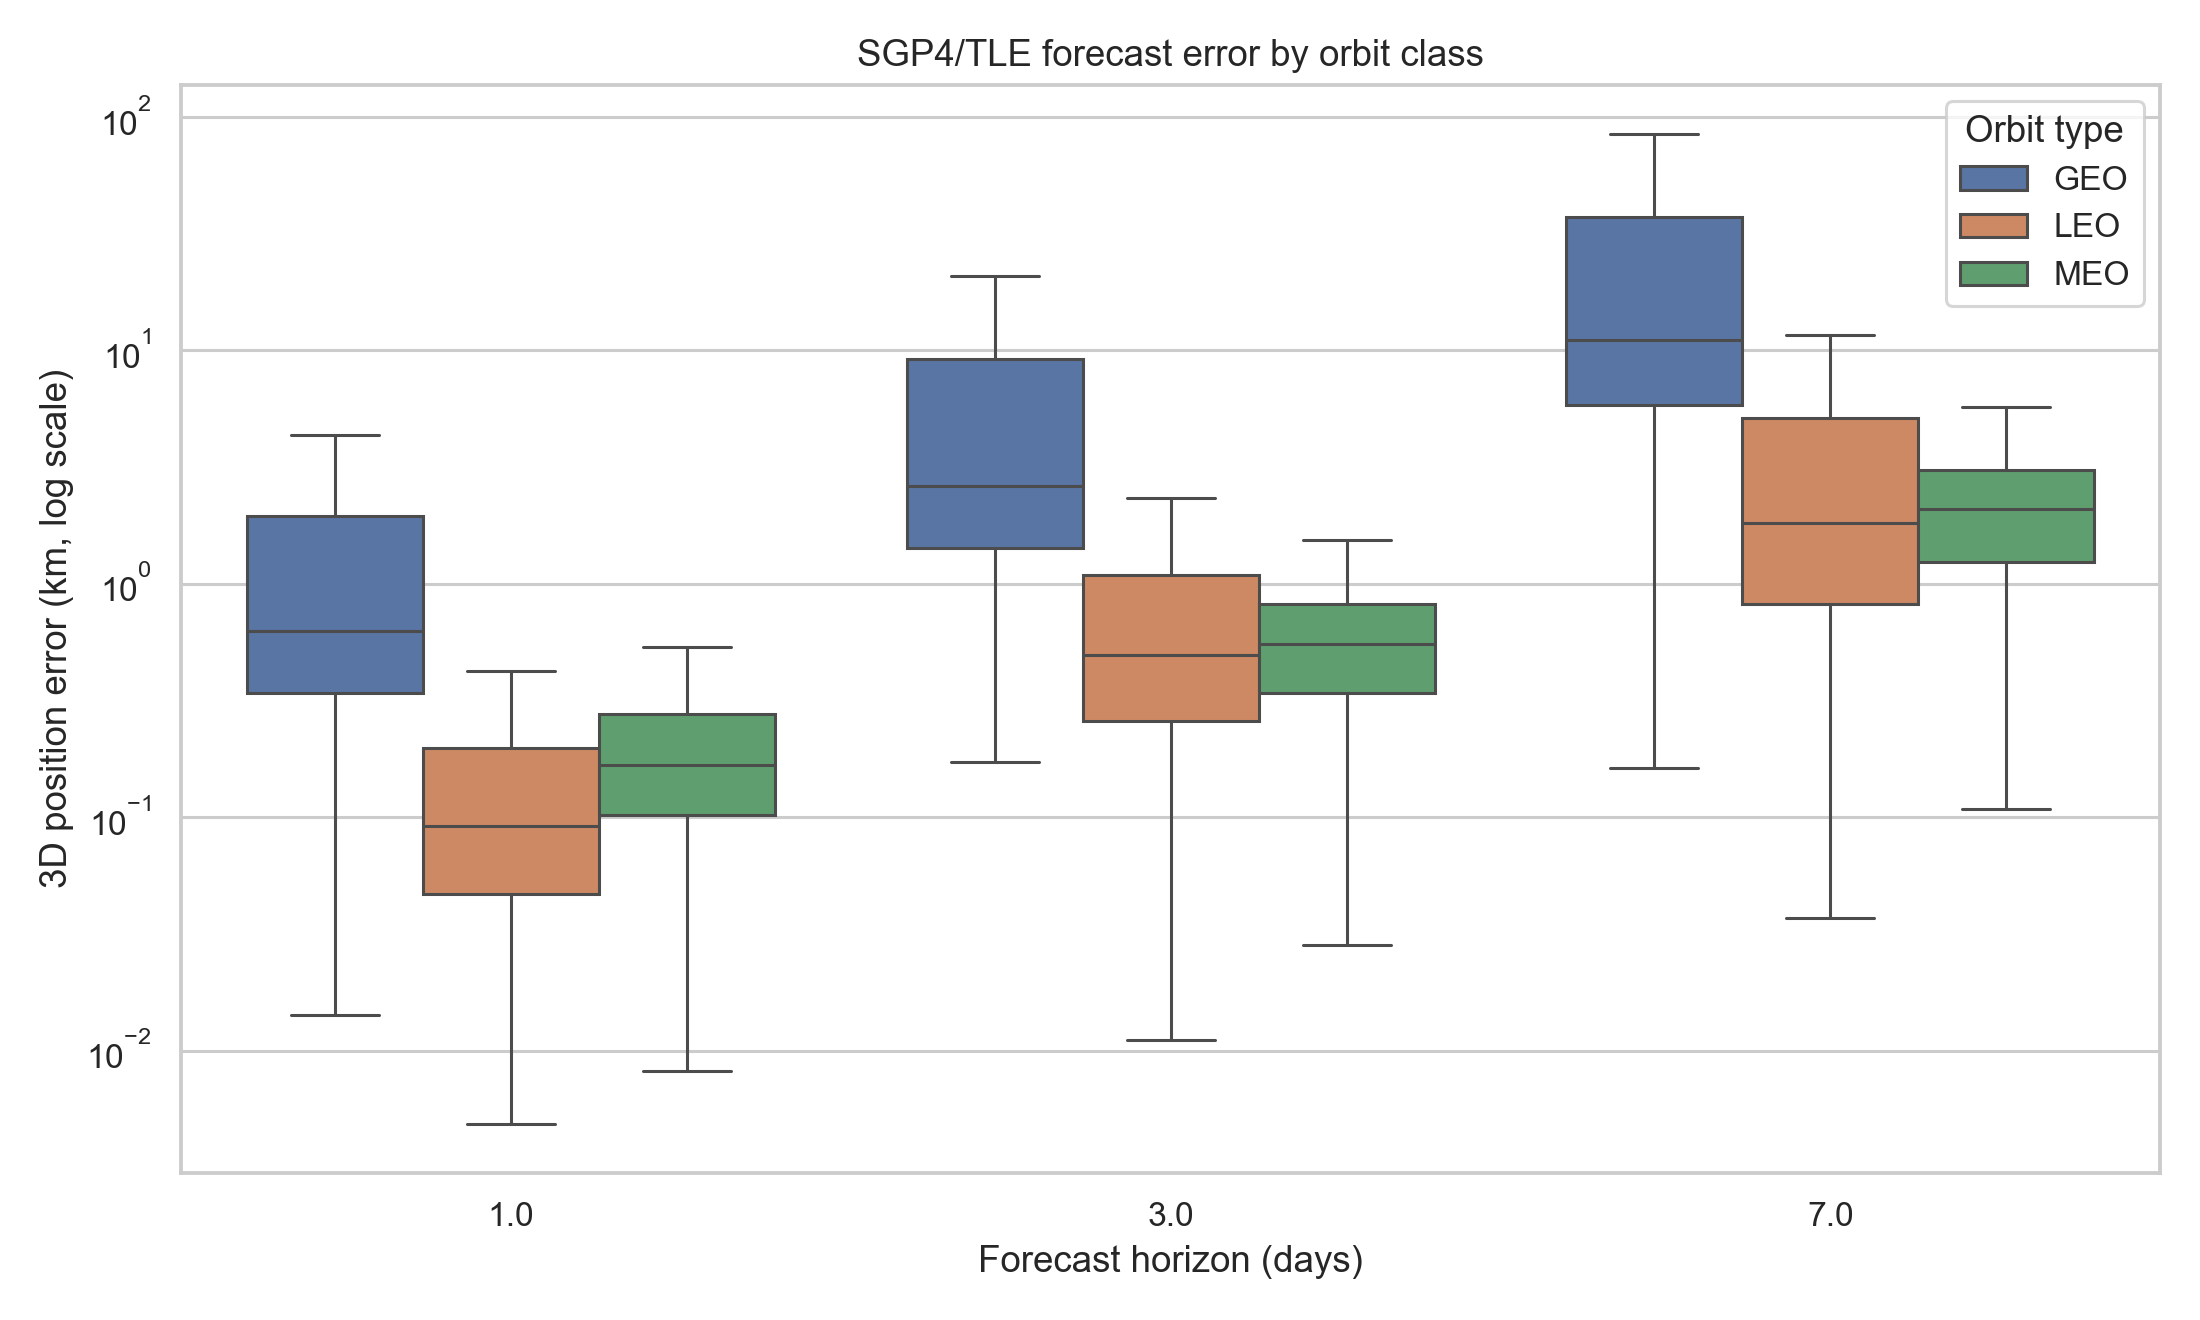
\includegraphics[width=0.9\linewidth]{../outputs/figures/error_boxplot_by_orbit_horizon.png}
\caption{不同轨道类型和预报时长的位置误差箱线图}
\end{figure}

\begin{figure}[htbp]
\centering
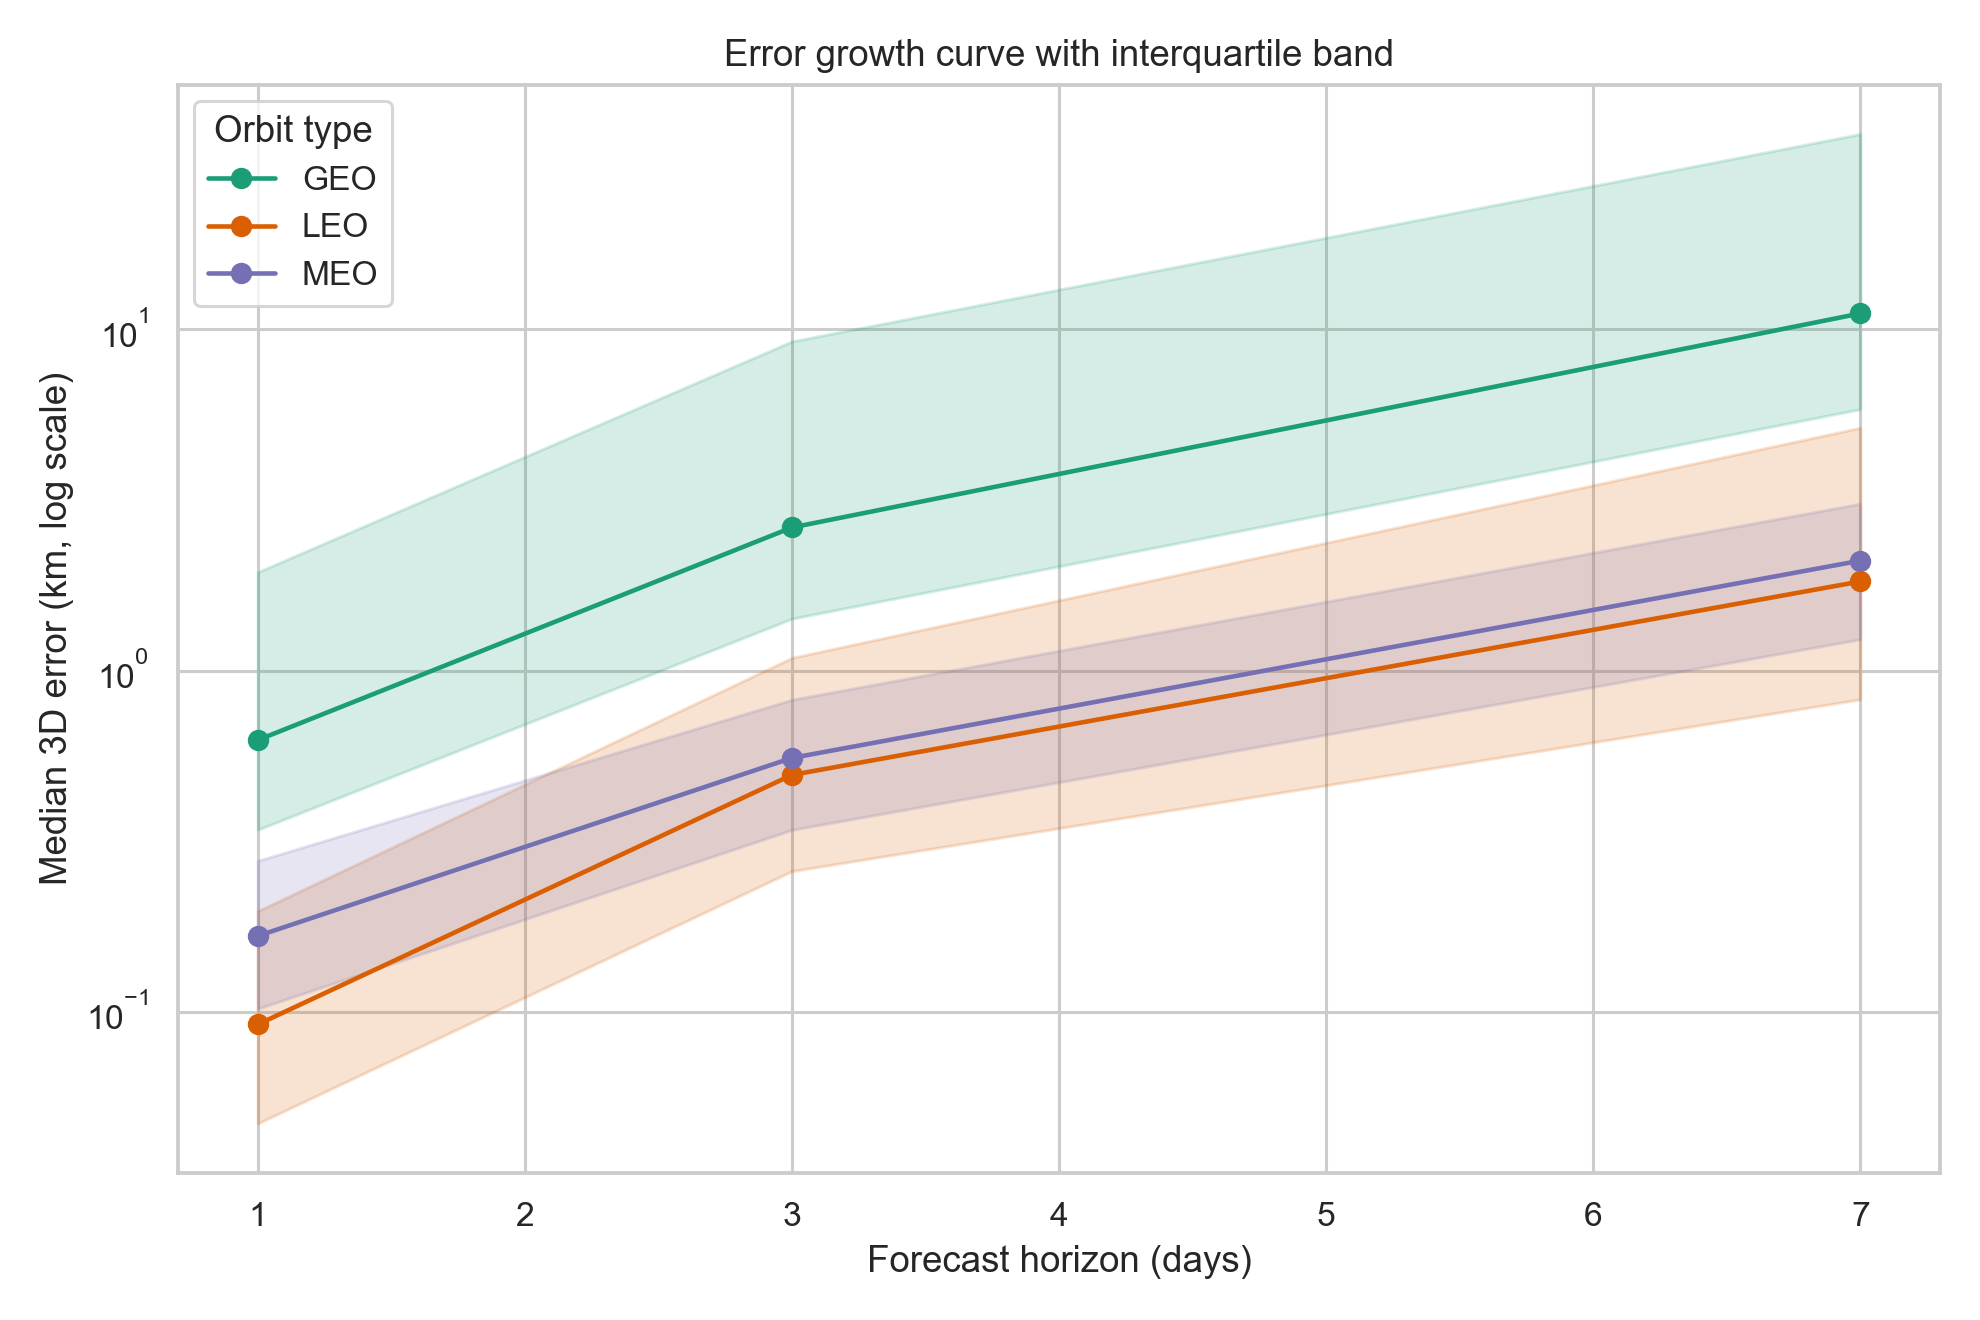
\includegraphics[width=0.9\linewidth]{../outputs/figures/error_growth_median_iqr.png}
\caption{误差增长曲线}
\end{figure}

\section{讨论}

讨论LEO大气阻力、MEO相位误差、GEO定点保持或机动等因素对误差增长的影响，并说明新TLE并非严格真值，因此本文估计的是旧TLE预报相对于新TLE后验轨道的近似误差。

\section{结论}

总结1/3/7天误差量级、误差增长律、轨道类型差异，以及Bootstrap区间相对于Gaussian近似的优势。

\end{document}
